% in clustering after dim red

Dimensionality reduction was implemented to reduce the number of dimensions (number of attributes, so in this case number of columns). Principal Components Analysis (PCA) and t-SNE, as described in section \ref{section:DimensionalityReduction}, were used to reduce the dimensionality of the data set. 

\subsubsection{PCA}
PCA was the initial approach used in the experiment. The sklearn PCA\footnote{\url{https://scikit-learn.org/stable/modules/generated/sklearn.decomposition.PCA.html}} function was used to reduce the number of dimensions to 2, which simplified visualisation in 2D scatterplots. The PCA allowed 65\%-95\% (depending on data preparation type) of the data's important structures to be accounted for in only the first two or three principle components. As can be seen in figure \ref{figure:PCA}a, the resulting data from these components, didn't show any significant clusters, in comparison to the t-SNE results. The principle components were further depicted in a 3D scatter plot, in the hopes that the extra dimension reveal more structure. However, as can be seen in \ref{figure:PCA}b, the results were practically the same.

\begin{figure}[H]
  \centering
  \begin{subfigure}{.475\textwidth}
    \centering
    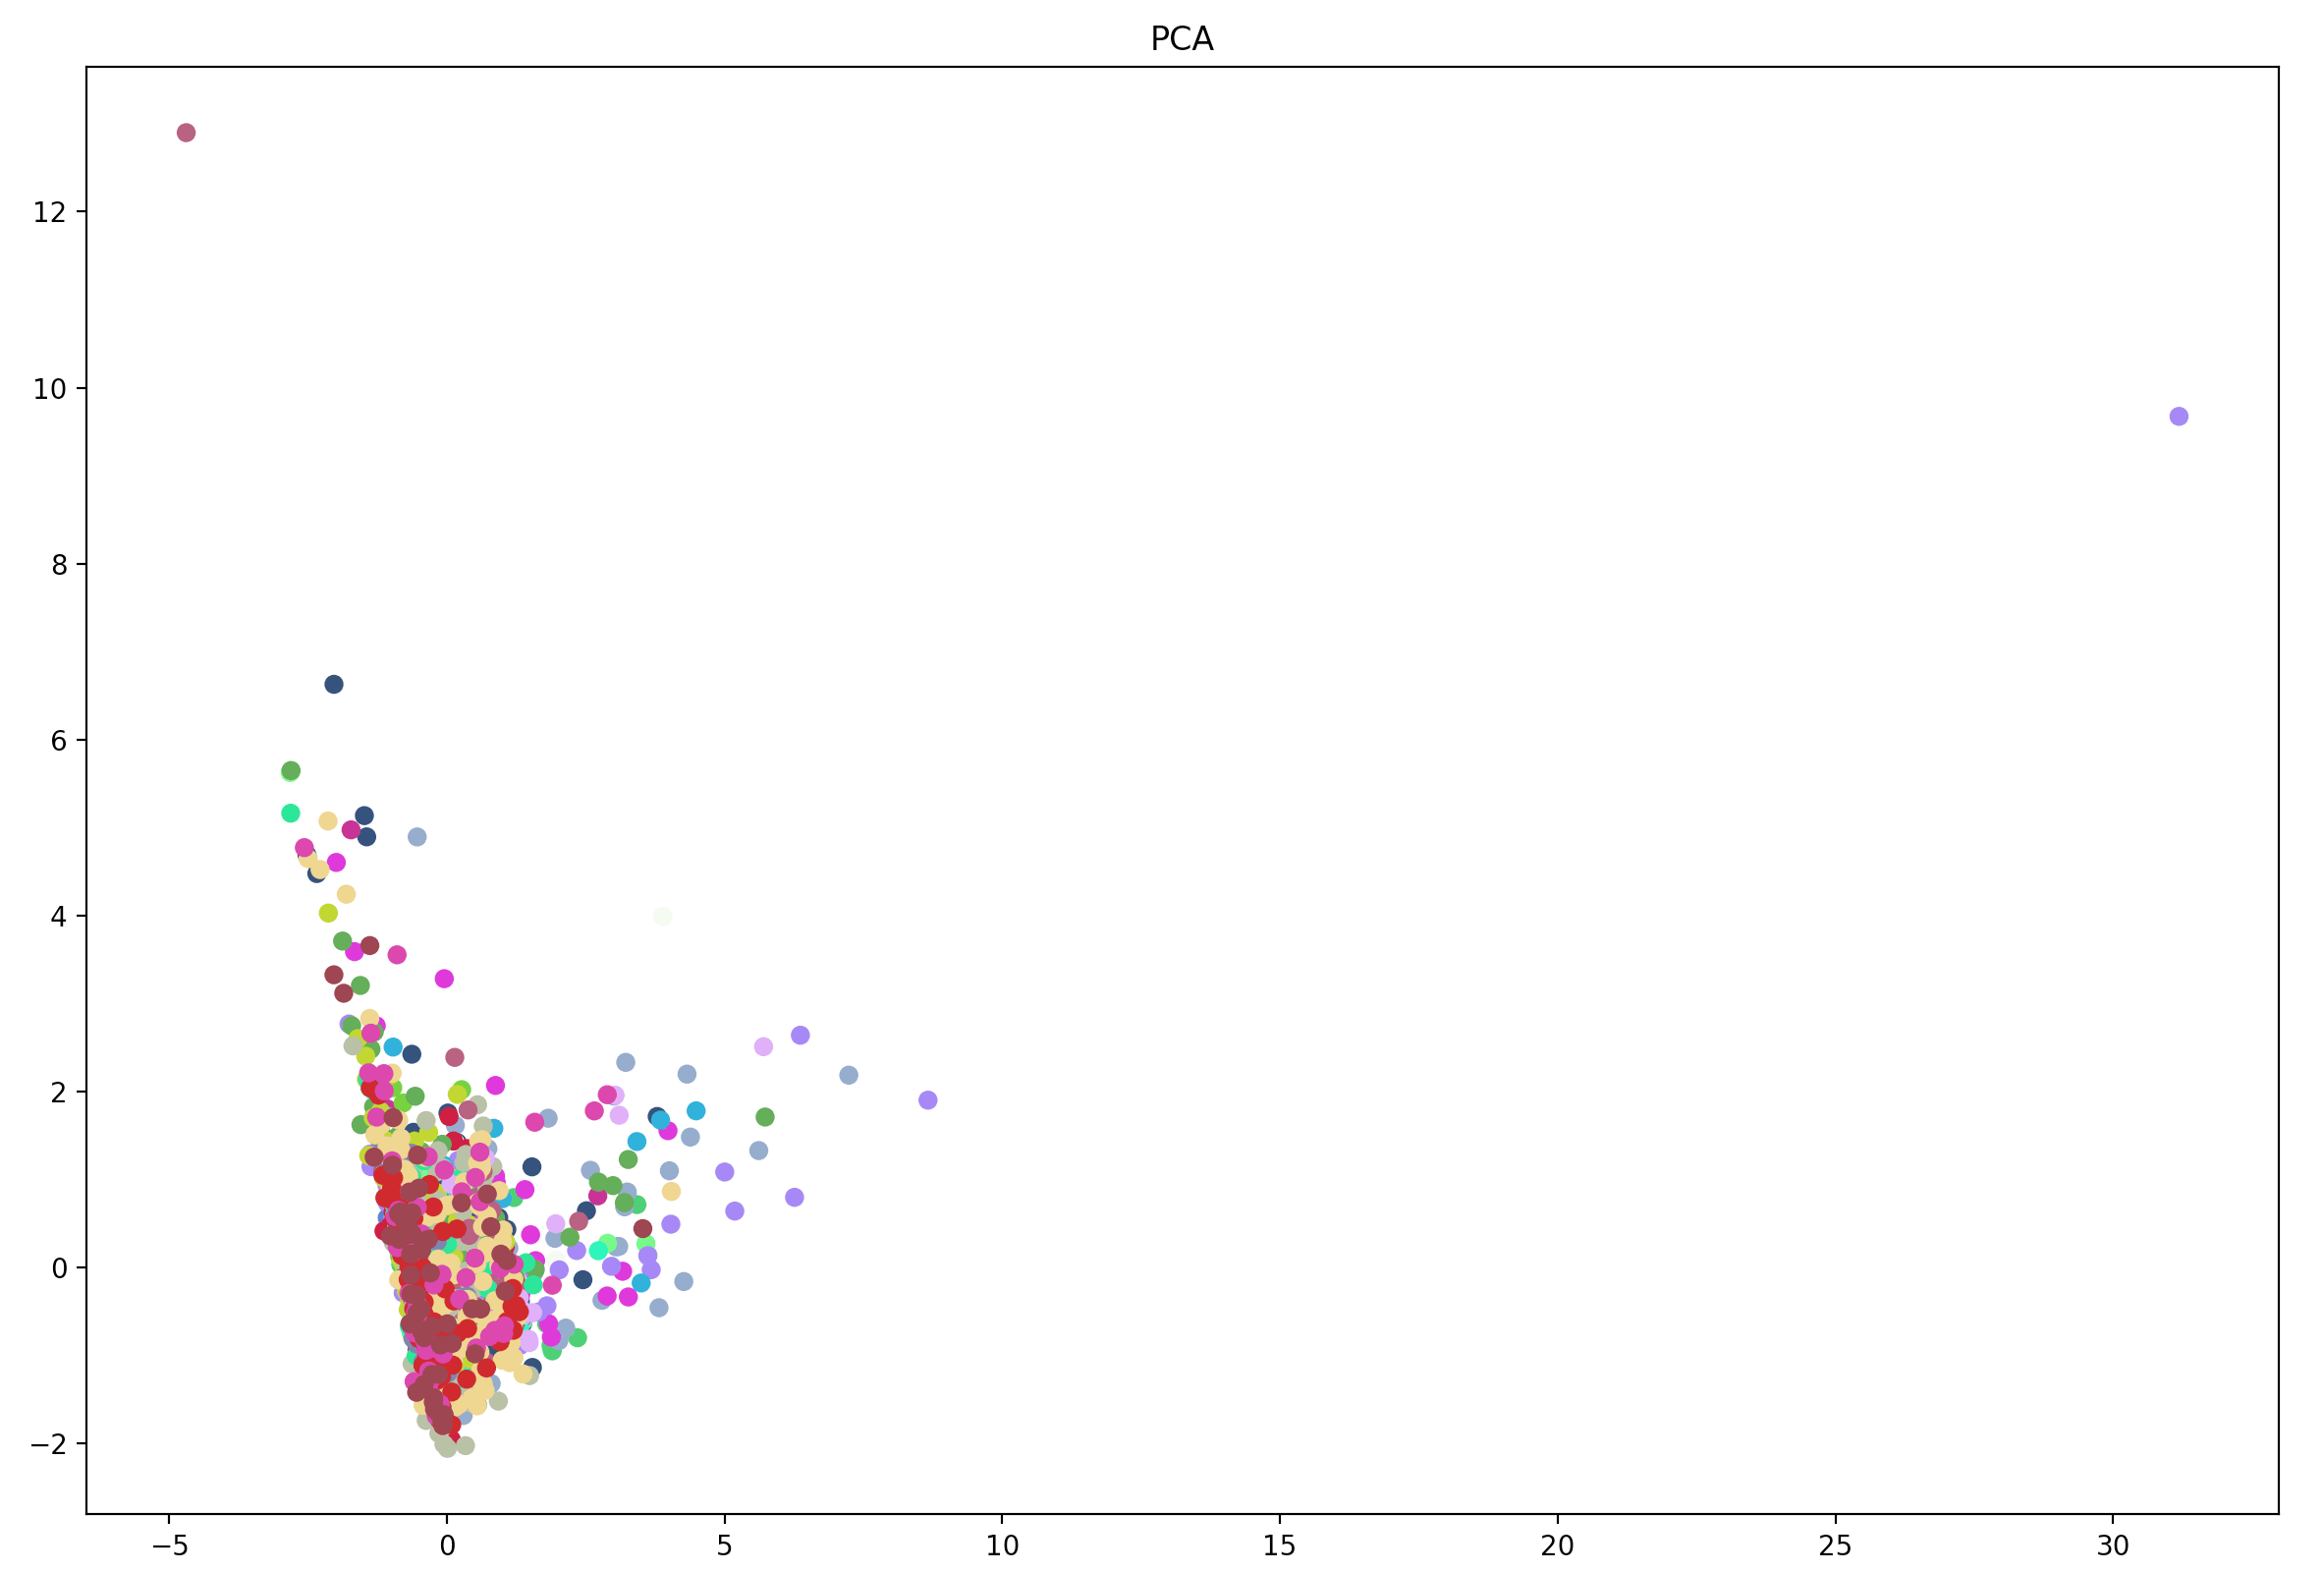
\includegraphics[width=1\textwidth]{./images/pca2d.png}
    % \caption{2D scatter plot with the PCA results. It only appears to form one cluster.}
    % \label{figure:}
  \end{subfigure}%
  \hfill
  \begin{subfigure}{.475\textwidth}
    \centering
    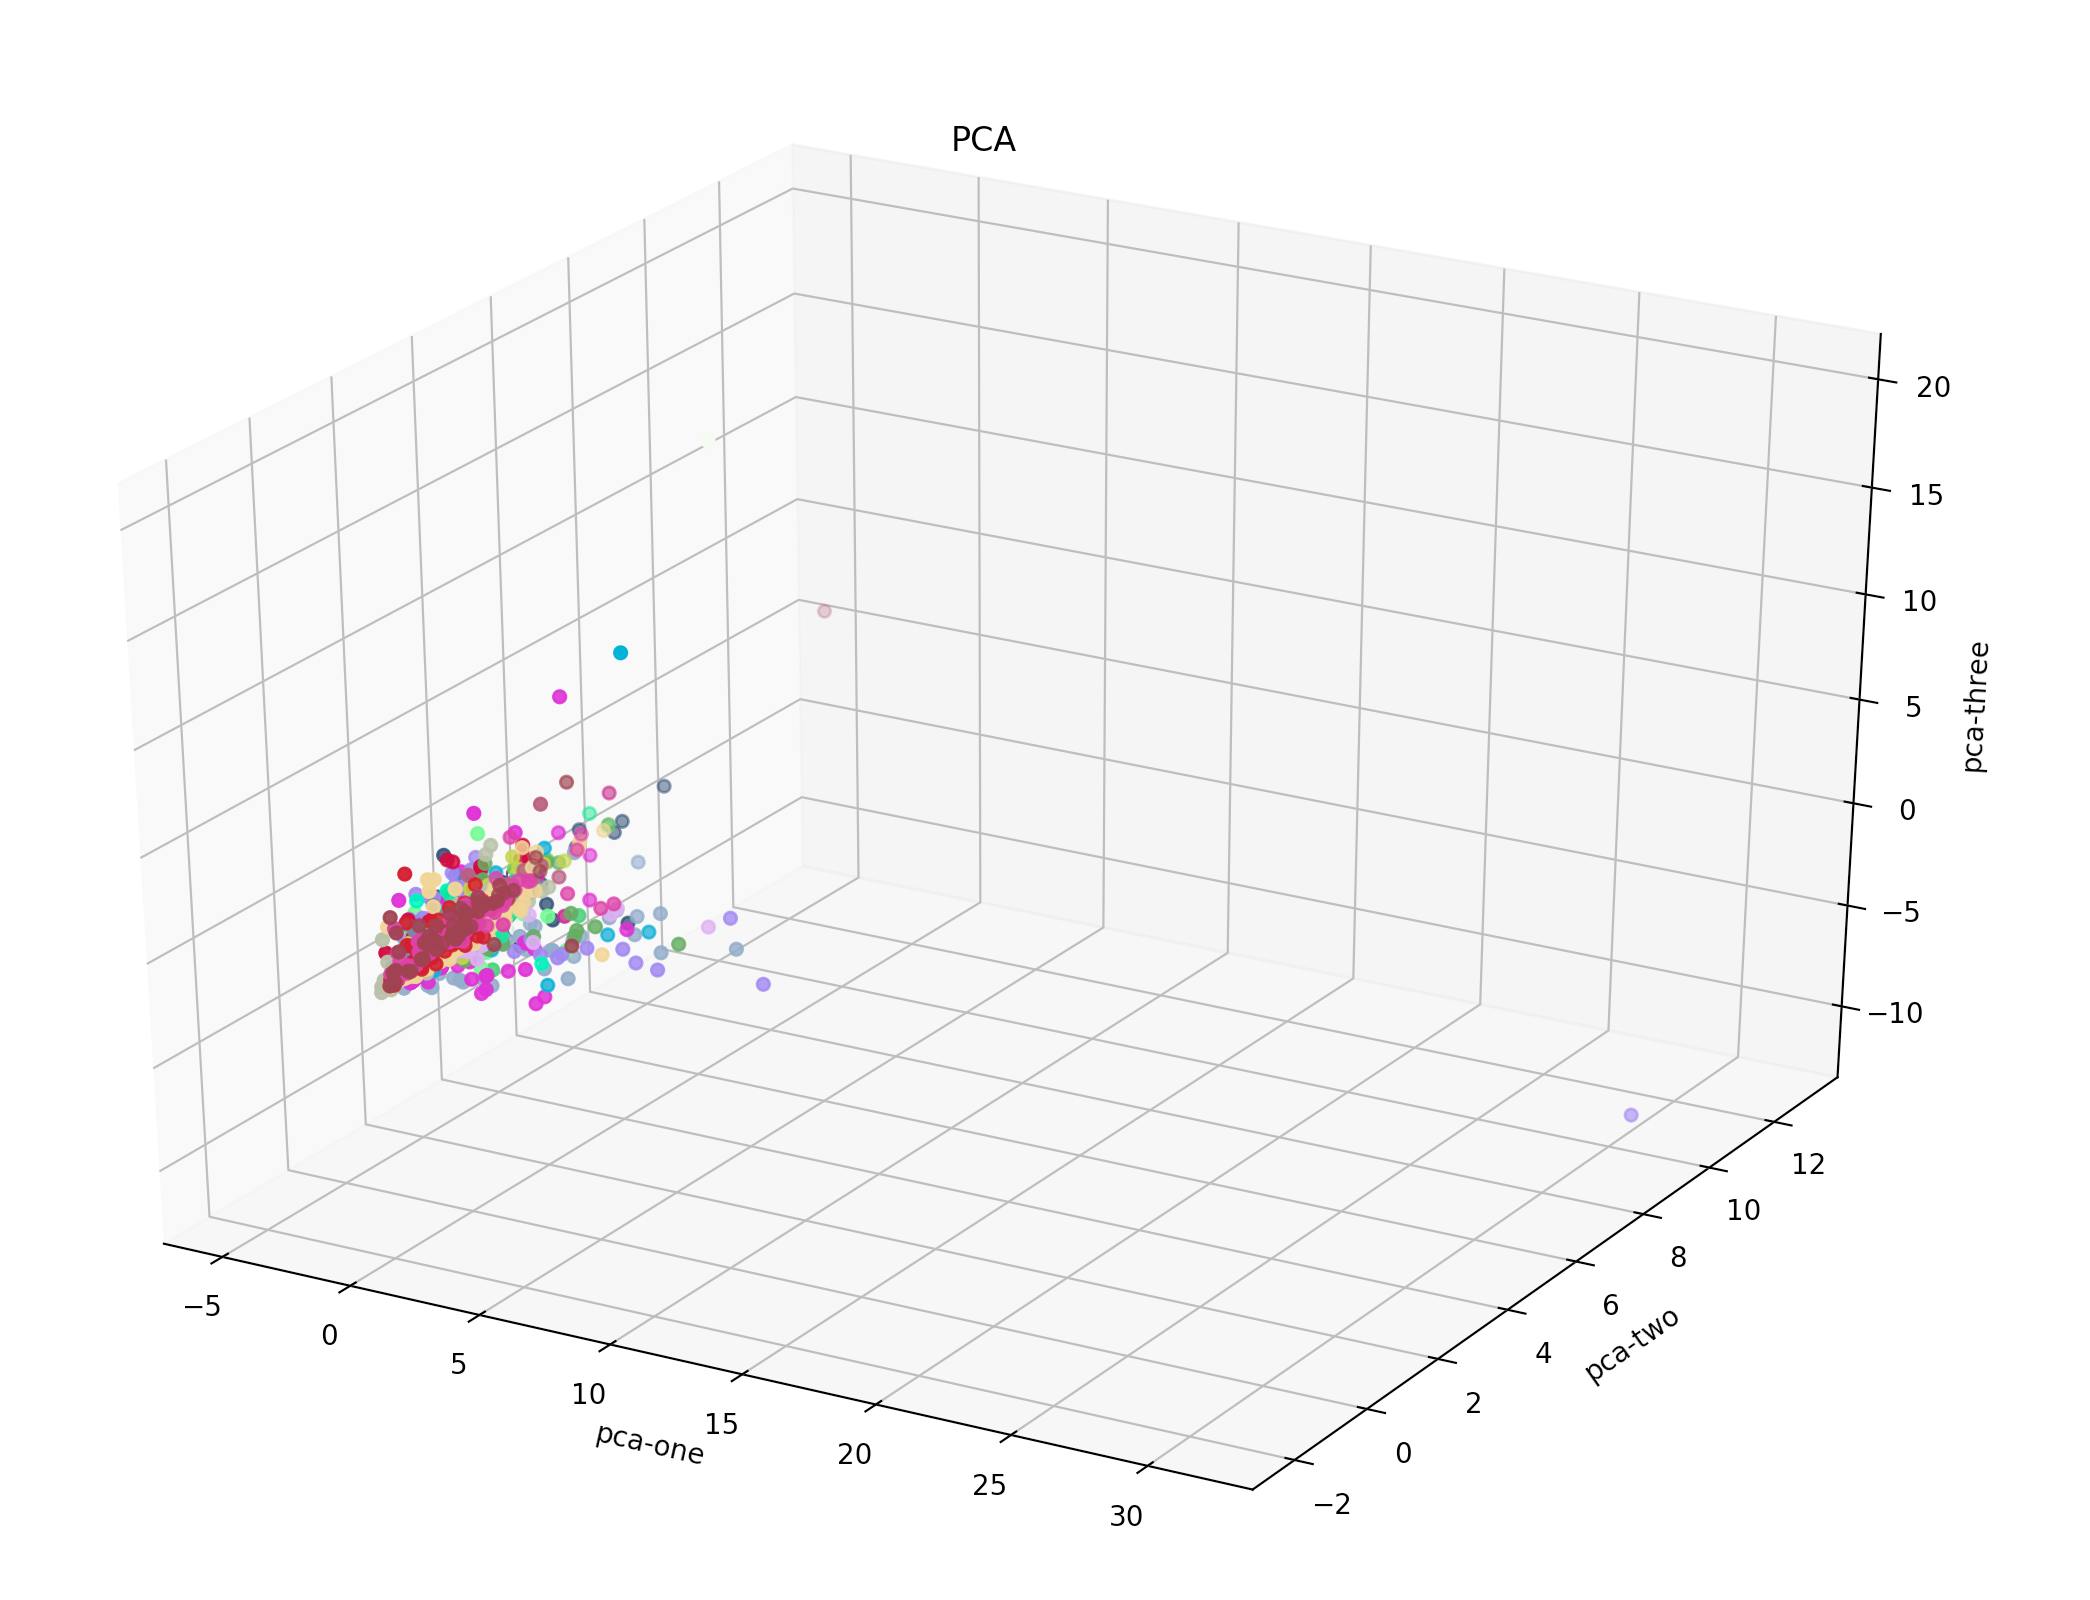
\includegraphics[width=1\textwidth]{./images/pca3d.png}
    % \caption{3D scatter plot with the PCA results. It only appears to form one cluster.}
    % \label{figure:}
  \end{subfigure}
	\caption{2D (a) and 3D (b) scatter plots of the PCA results. The data points only appear to form one cluster with little visible structure.}
  \label{figure:PCA}
\end{figure}
%&todo - this is because not linear data and pca is linear.
%todo - mention 3D or just stick to 2D



\subsubsection{t-SNE}
% \subsubsection{Find t-SNE parameters}
The t-SNE algorithm was implemented using the sklearn t-SNE\footnote{\url{https://scikit-learn.org/stable/modules/generated/sklearn.manifold.TSNE.html}} method.
To be able effectively apply the t-SNE algorithm, it was important to identify the parameters (perplexity, learning \textbf{todo: what is the learning rate}, and number of iterations) most suitable to the SmartEater data set, as described in section \ref{section:tSNE}. The number of iterations was originally set to the default value 1000, but was later raised to 5000, to avoid receiving significantly different results each time t-SNE was run. Raising the number of iterations provided more consistent results. The overall structure of these were the same, though usually rotated differently. 5000 iterations was also used in the experiments by \textcite{wattenberg2016how}, who claimed that their t-SNE plot had reached a stable point by then.

To find suitable perplexity and learning rate t-SNE parameters to create the most distinct clusters possible, multiple results created using various parameter values were compared. For this, 2D t-SNE scatter plots were created using different perplexity and learning rate values. 
First to the perplexity. \textcite{wattenberg2016how} proved to be a helpful source in tuning this parameter. Multiple values between the recommended 5 and 50 were tested. The resulting scatter plots are listed in the appendix \ref{appendix:tSNEParametersPerplexity}. The graphs on the left depict the t-SNE results, while the scatter plots on the right illustrate DBSCAN clustering of these results. The DBSCAN cluster colourings were placed here to support in perceiving the differences between the t-SNE structured data. When visually comparing the different perplexities, the data points in the lower perplexity graphs (e.g. 5 and 10) appear to be randomly scattered and have no stucture. The higher the perplexity gets, the more the data points take on structure and more distinct and well defined clusters appear. From perplexity 20, the one hour data files appear to start forming such clusters. When scanning the higher perplexities, it can be seen that clusters become more separated. The scatter plots from perplexity 30 to 50 appear to have formed well defined clusters. 

To aid in selecting the perplexity that creates the best clusters, the three mathematical evaluation scores mentioned in section \ref{section:TheoryEvaluatingClusteringResults} were compared. Figure \ref{figure:perplexityEvaluationScores} displays the Silhouette Coefficient, Davies-Bouldin Index, and Caliński-Harabasz Index were calculated for the DBSCAN and OPTICS clusterings of different perplexities. The light green highlighted values illustrate the best values (best defined and distinct clusters) for the one hour or three hour time lengths, whilst the darker green features the overall best value. With 4, a perplexity of 20 has the highest number of best achieving score values, 10, 40, and 45 tying in second place with 2. While according to the scores, perplexity 20 creates the best clusters, visually the clusters appear better defined from with a perplexity 30 to 50. For this reason, the focus of the comparison of the scores was moved to the scores that came second and whose perplexity was between 30 and 50. Perplexity 40 is a clear winner in figure \ref{figure:perplexityEvaluationScoresDetailed} and was chosen as the final parameter. These tests were conducted a second time (see appendix \ref{compareAveragePerplexity}), using the average of two different t-SNE results for each time length (1h and 3h). While the scores are slightly different, a perplexity of 40 was again the overall result.
% Comparing these results with the scatter plots and allowing for error, the 

To further confirm the t-SNE perplexity parameter, the equation reviewed in section \ref{section:tSNE} was implemented. However, the results were not as expected and so the results from the visual and evaluation score comparison were chosen.

% The first block (\textbf{lines...}) shows the results for the 1h data set, the second block (\textbf{lines...}) for the 3h data set, and the last block (\textbf{lines...}) compares the two (for the 1h and 3h time lengths). The light green field indicates, that from the data files (1h or 3h), this time length achieved the best and most distinct clusters, according to that score. Dark green fields highlight the best value for that score overall for all time lengths.

\begin{figure}
  \centering
  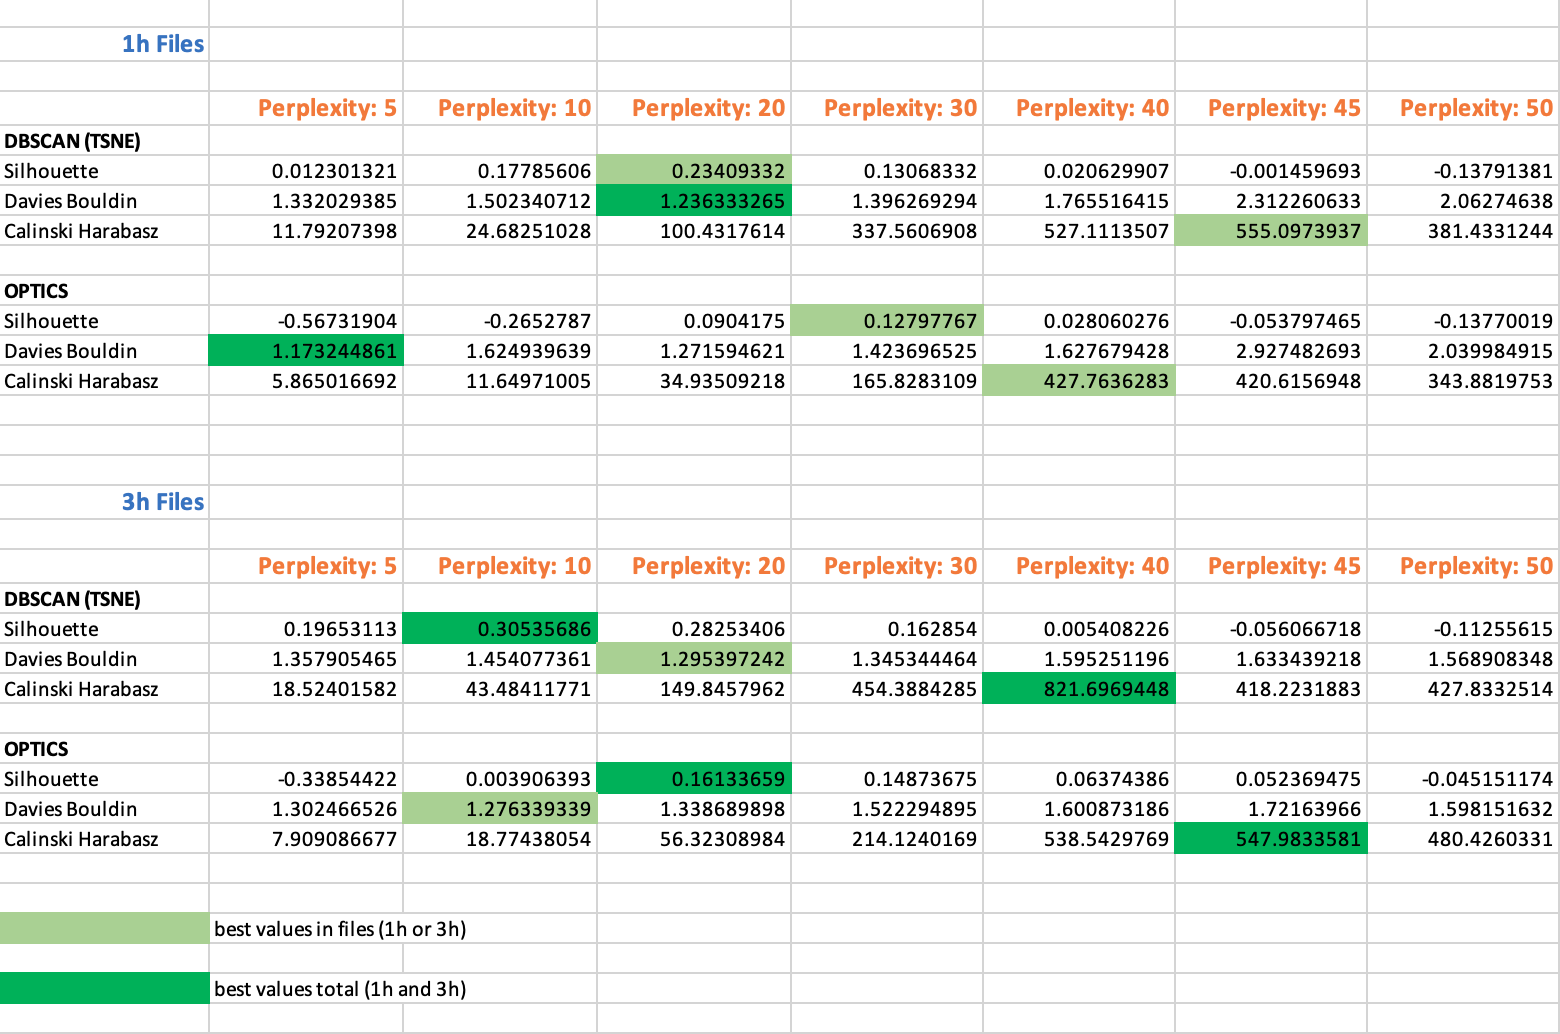
\includegraphics[width=0.8\textwidth]{./images/tsneParametersTest/perplexity/perplexityEvaluationScores.png}
  \caption{Comparison of Silhouette Coefficient, Davies-Bouldin Index, and Caliński-Harabasz Index for different t-SNE \textbf{perplexities}.}
  \label{figure:perplexityEvaluationScores}
\end{figure}

\begin{figure}
  \centering
  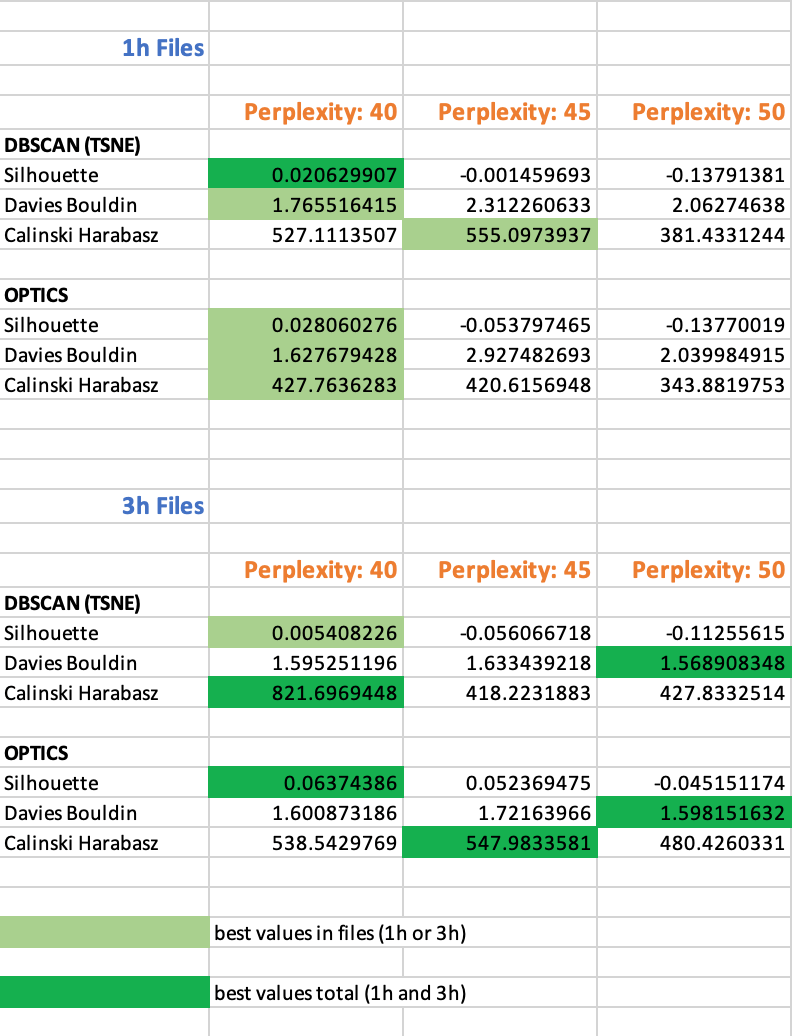
\includegraphics[width=0.4\textwidth]{./images/tsneParametersTest/perplexity/perplexityEvaluationScoresDetailed.png}
  \caption{Comparison of Silhouette Coefficient, Davies-Bouldin Index, and Caliński-Harabasz Index for different t-SNE \textbf{perplexities}.}
  \label{figure:perplexityEvaluationScoresDetailed}
\end{figure}


The same principle was used to determine the ideal value for the learning rate parameter.  The sklearn t-SNE documentation states, that the learning rate is normally set between 10 and 1000, hence the learning rate in the scatter plots was chosen in this interval.
The various resulting scatter plots can be seen in the appendix \ref{appendix:tSNEParametersLearningRate}. The differences in the arrangement of the data points over the plots is not as substantial as it was when testing for the perplexity. The results, listed in figure \ref{figure:learningRateEvaluationScores} reveal, that the learning rate 10 scores highest with a learning rate of 800 coming in second. Since roughly 200 steps were taken when testing the learning rate value, smaller steps were taken (i.e. 50) around the winning value to see if an even better performance could be accomplished (figure \ref{figure:learningRateEvaluationScoresDetailed}). While 10 still achieved best in the one hour time length files, 800 came top in the three hour files, indicating that 10 might not be the best rate for these. Consequently, the values 20 and 30 were also evaluated (figure \ref{figure:learningRateEvaluationScoresDetailed2}). While a learning rate of 10 still came top in the one hour files, 30 came top in the three hour files. With the hope of finding a value in between 10 and 30 that satisfied both time lengths, the learning rates 10, 15, 20, 25, and 30 were ultimately compared exclusively. The results in figure \ref{figure:learningRateEvaluationScoresDetailed3} reveal, that this final comparison lead to the learning rate 20 being the most suitable. As with the perplexity, the learning rate tests were also reproduced, averaging two different t-SNE outcomes. The results are illustrated int appendix \ref{appendix:compareAverageLearningRate}. In general, the results are similiar. 800 appears to more dominant than the lower parameter values (e.g. 10 and the favourite 20). To further compare 20 and 800, appendix \ref{appendig:compareLearningRate20and800} contains a table (figure \ref{figure:learningRateEvaluationScoresAverageDetailed4}) comparing 4 different runs of scores from average t-SNE results. With 2 wins more than 20, 800 has the overall better score results. Figures \ref{figure:1h-learningRateComparison20and800} and \ref{figure:3h-learningRateComparison20and800} visually compare the scatter plots created with a learning rate of 20 and 800. The plots and clusters appear very similar. The clusters from perplexity 20 however seem slightly more compact (less smaller clusters). A learning rate of 20 was thus selected for the final learning rate parameter.

% These tests were conducted a second time (see apendix \textbf{todo}), using the average of two different t-SNE results for each time length (1h and 3h). While the scores are slightly different, a perplexity of 40 was again the overall result.

The final t-SNE parameters, from which the results were then used by the DBSCAN and OPTICS clustering methods in the next section, were as follows: perplexity=40, learning\_rate = 20, and n\_iter=5000.


\begin{figure}
  \centering
  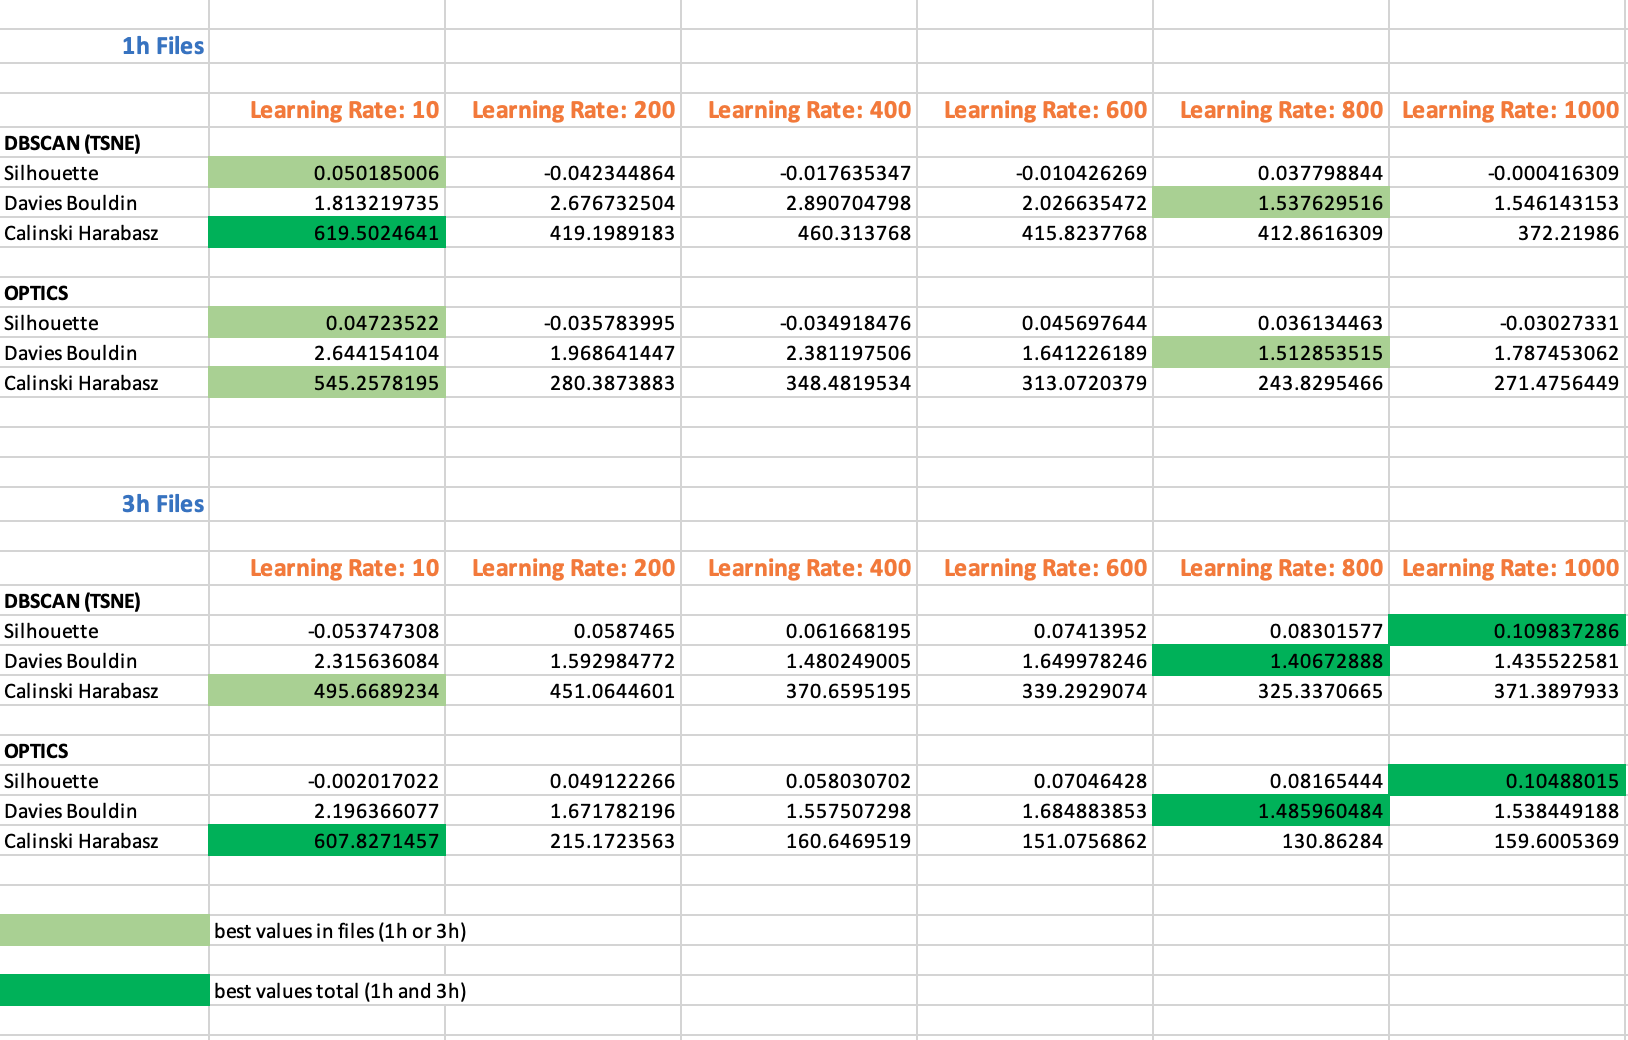
\includegraphics[width=0.8\textwidth]{./images/tsneParametersTest/learningRate/learningRateEvaluationScores.png}
  \caption{Comparison of Silhouette Coefficient, Davies-Bouldin Index, and Caliński-Harabasz Index for different t-SNE \textbf{learning rate} values.}
  \label{figure:learningRateEvaluationScores}
\end{figure}

\begin{figure}
  \centering
  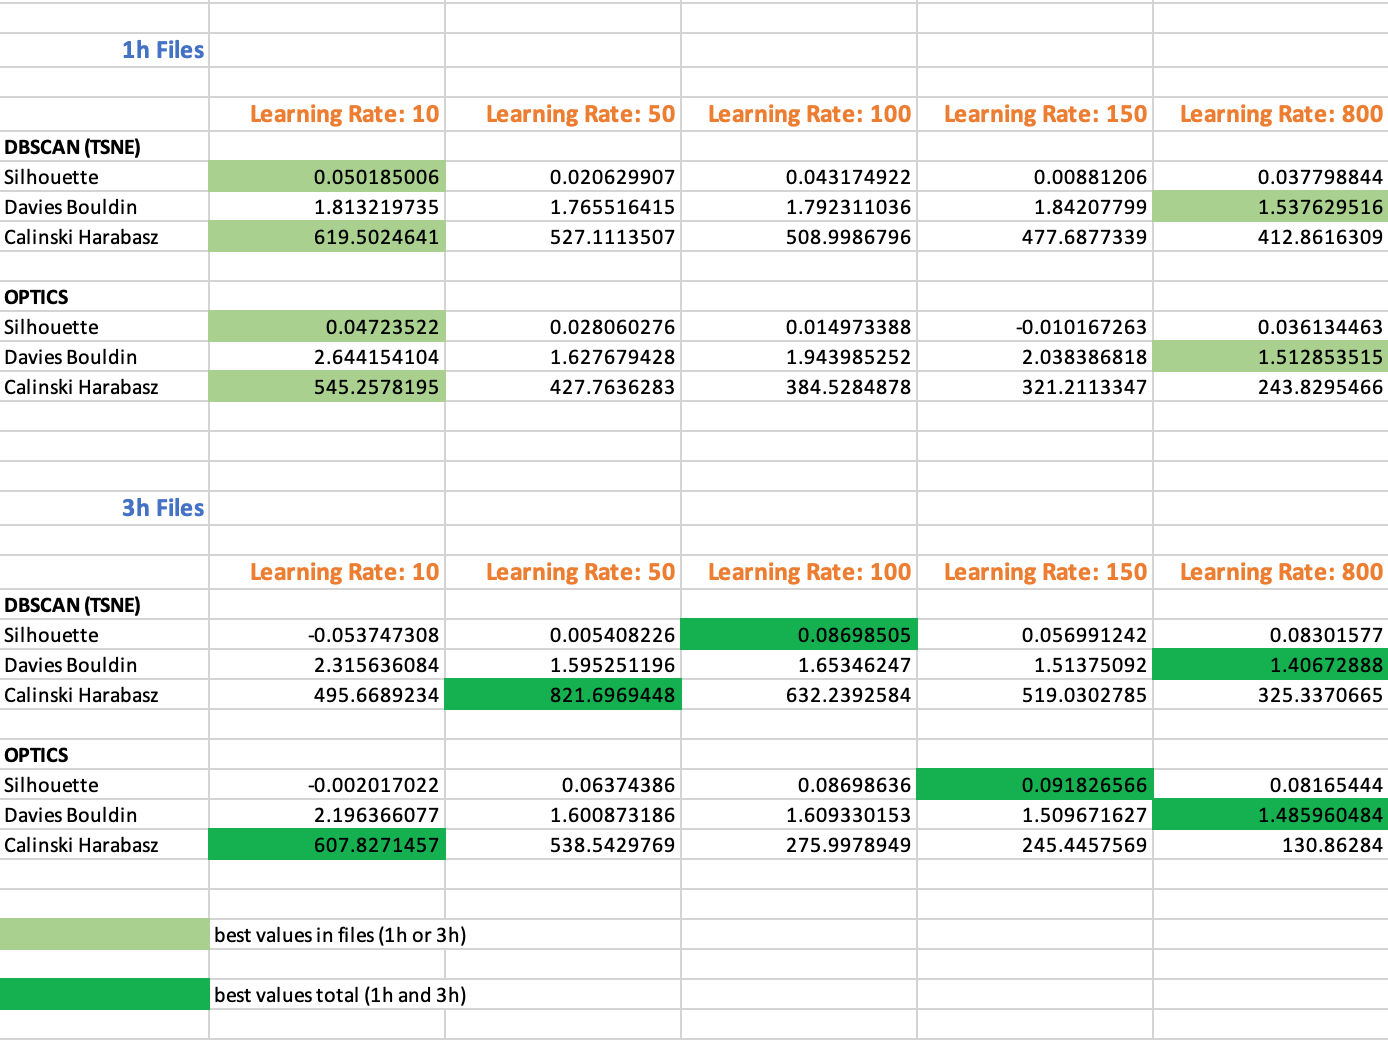
\includegraphics[width=0.8\textwidth]{./images/tsneParametersTest/learningRate/learningRateEvaluationScoresDetailed.png}
  \caption{Comparison of Silhouette Coefficient, Davies-Bouldin Index, and Caliński-Harabasz Index for different t-SNE \textbf{learning rate} values.}
  \label{figure:learningRateEvaluationScoresDetailed}
\end{figure}

\begin{figure}
  \centering
  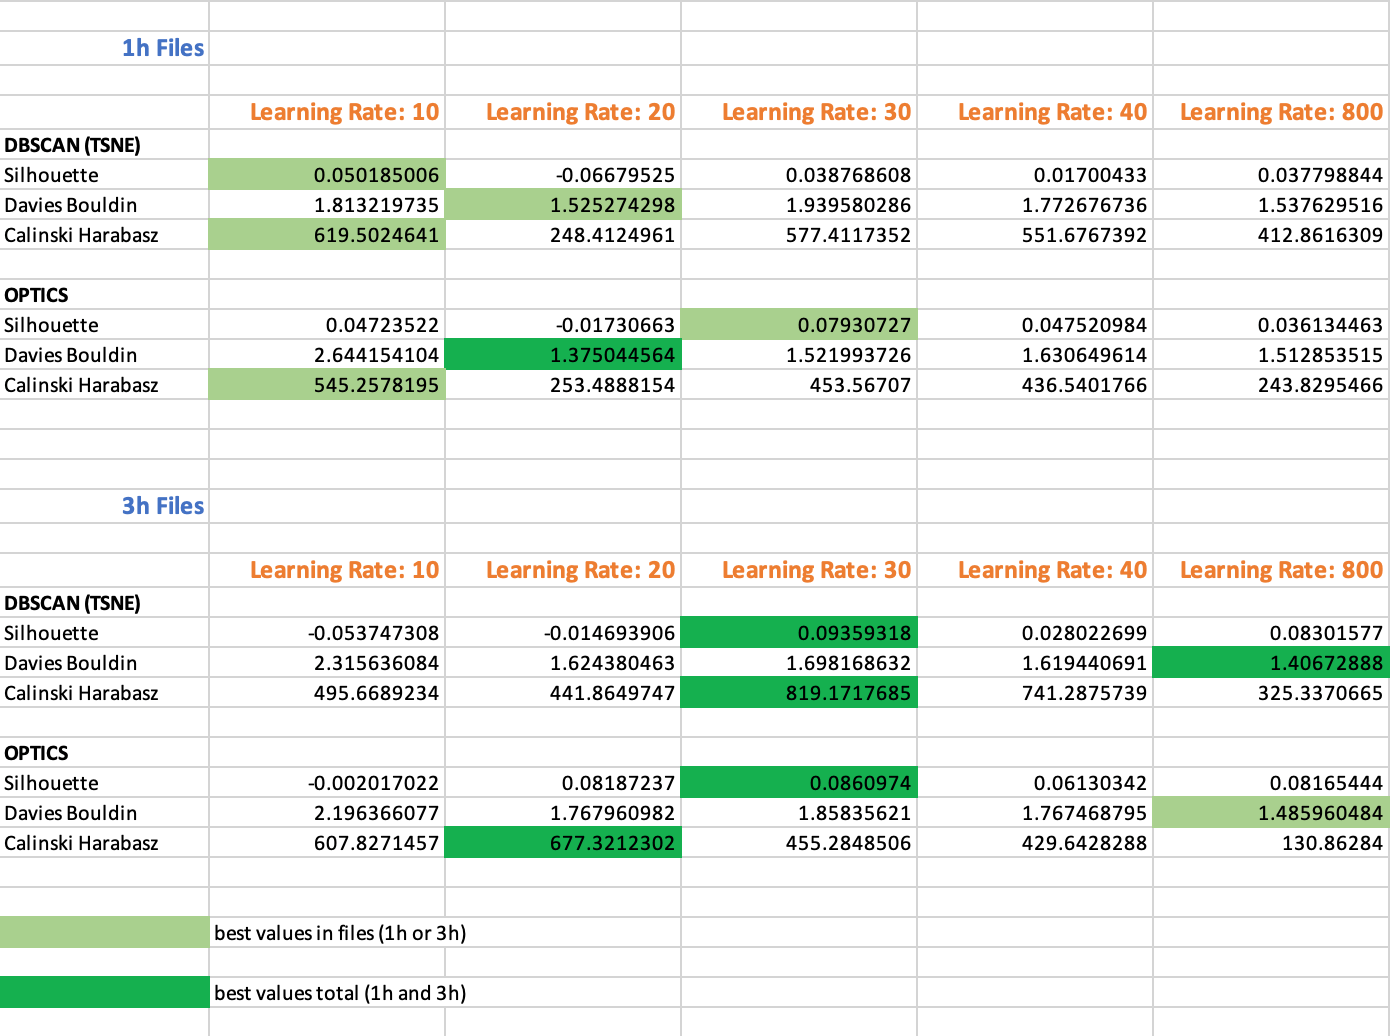
\includegraphics[width=0.8\textwidth]{./images/tsneParametersTest/learningRate/learningRateEvaluationScoresDetailed2.png}
  \caption{Comparison of Silhouette Coefficient, Davies-Bouldin Index, and Caliński-Harabasz Index for different t-SNE \textbf{learning rate} values.}
  \label{figure:learningRateEvaluationScoresDetailed2}
\end{figure}

\begin{figure}
  \centering
  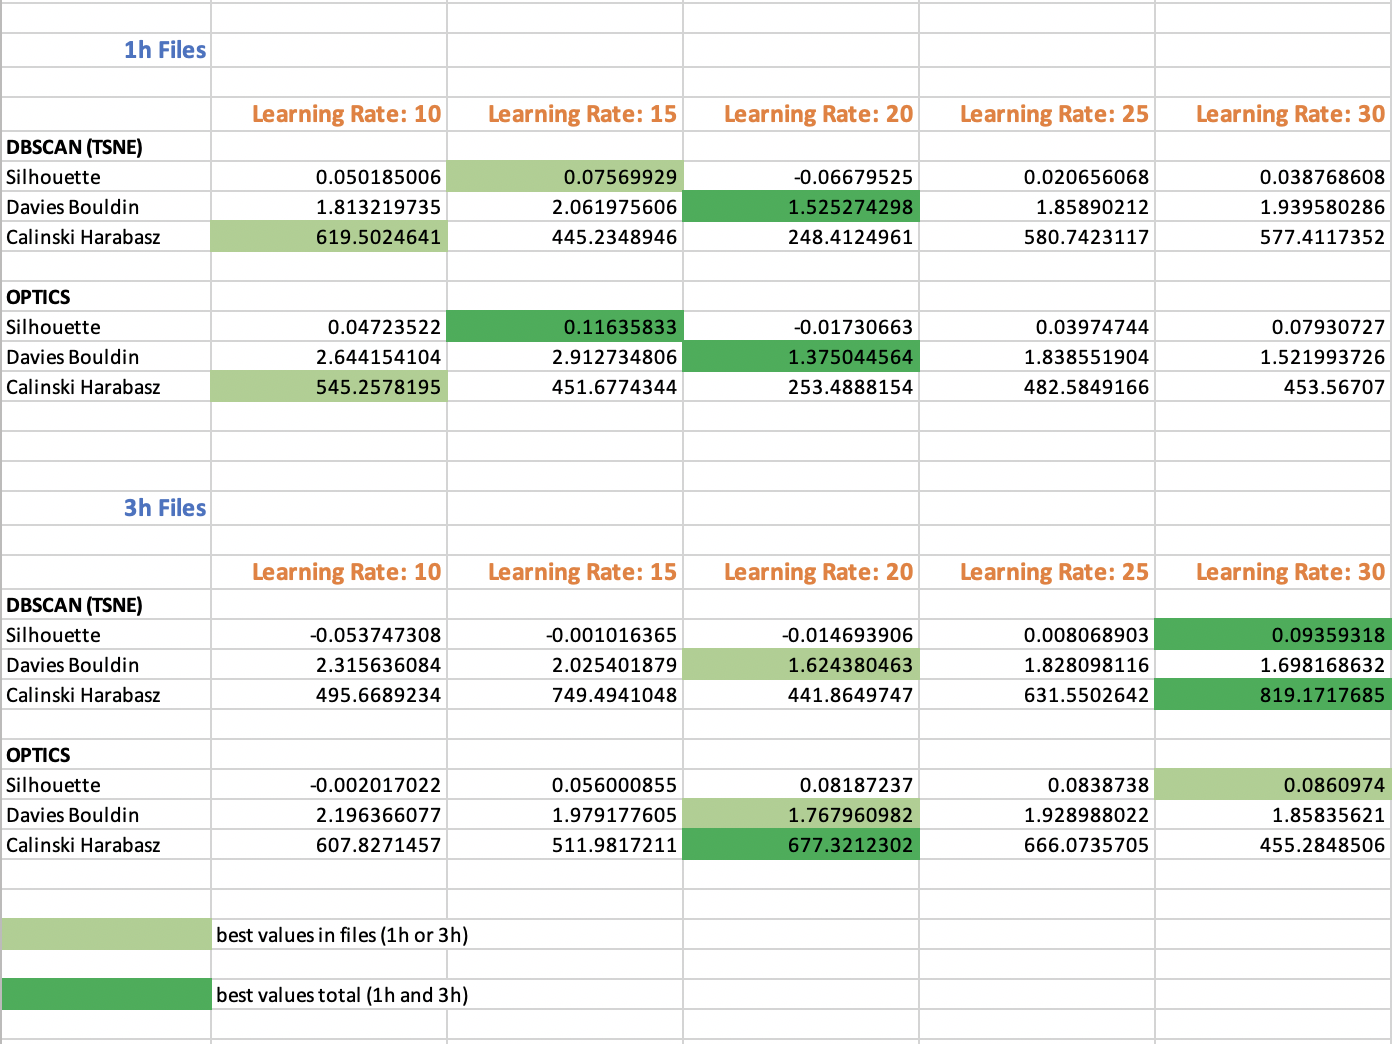
\includegraphics[width=0.8\textwidth]{./images/tsneParametersTest/learningRate/learningRateEvaluationScoresDetailed3.png}
  \caption{Comparison of Silhouette Coefficient, Davies-Bouldin Index, and Caliński-Harabasz Index for different t-SNE \textbf{learning rate} values.}
  \label{figure:learningRateEvaluationScoresDetailed3}
\end{figure}





\clearpage
